\documentclass[aspectratio=169]{beamer}
\usepackage[utf8]{inputenc}
\usepackage{amsmath}
\usepackage{tikz}
\usepackage{opensans}

\title{Topology and Continuity}
\author{Paulo Fagandini}
\institute{\includegraphics[scale=0.3]{NovaPrincipalV1.png}}
\date{}

\makeatletter
\setbeamertemplate{theorem begin}{%
  \setbeamercolor{block title}{bg=white,fg=black}%
  \setbeamercolor{itemize item}{fg=black}%
  \setbeamercolor{itemize subitem}{fg=black}%
  \setbeamercolor{itemize subsubitem}{fg=black}%
  \setbeamercolor{enumerate item}{fg=black}%
  \setbeamercolor{enumerate subitem}{fg=black}%
  \setbeamercolor{enumerate subsubitem}{fg=black}%
  \begin{\inserttheoremblockenv}
    {%
      \textbf{\inserttheoremname}
      %\inserttheoremnumber
      \ifx\inserttheoremaddition\@empty\else\ \inserttheoremaddition\fi%
    }%
    \normalfont%
}

\setbeamertemplate{theorem end}{%
    \end{\inserttheoremblockenv}%
}

\setbeamercolor{block title}{bg=white,fg=black}%
\setbeamercolor{itemize item}{fg=black}%
\setbeamercolor{itemize subitem}{fg=black}%
\setbeamercolor{itemize subsubitem}{fg=black}%
\setbeamercolor{enumerate item}{fg=black}%
\setbeamercolor{enumerate subitem}{fg=black}%
\setbeamercolor{enumerate subsubitem}{fg=black}%

\makeatother

\newtheorem{defenition}{Definition}[section]
\newtheorem{proposition}{Conjecture}[section]

\AtBeginSection{\frame{\sectionpage}}

\setbeamertemplate{footline}{
    \hspace{0.05\textwidth}
    \raisebox{3ex}{\insertshortauthor{}}\hfill
    \raisebox{3ex}{\insertframenumber{}/\inserttotalframenumber} \hfill
    {\raisebox{3ex}{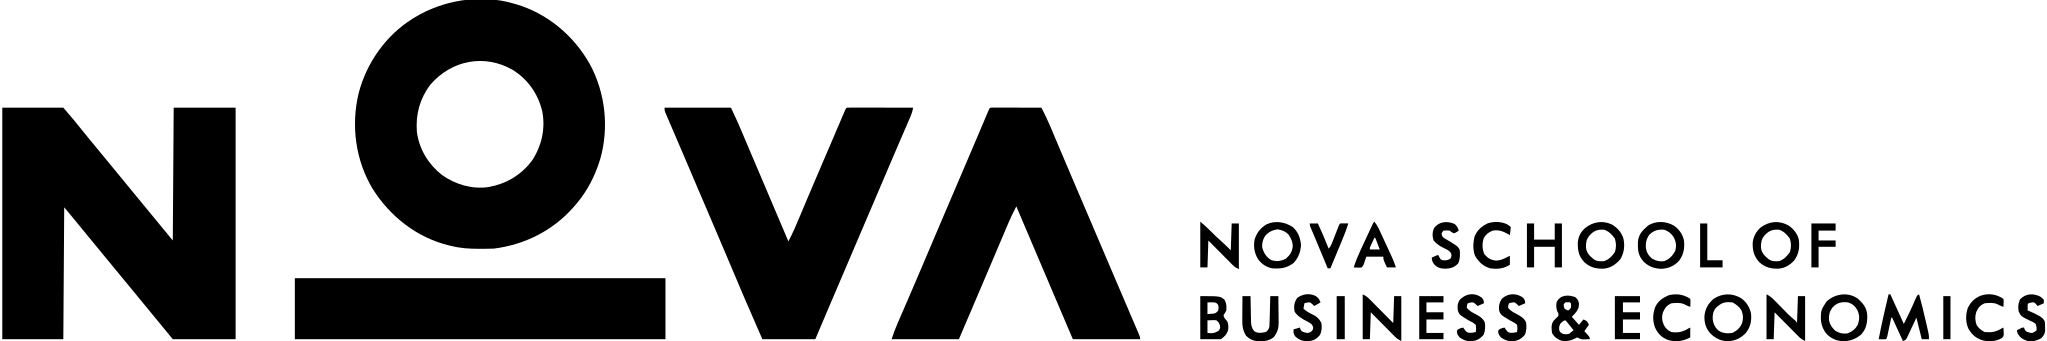
\includegraphics[height=0.04\textheight]{NovaPrincipalV2.png}}}
    \hspace{0.05\textwidth}
}

\setbeamertemplate{navigation symbols}{}

\setbeamercolor{title}{fg = black}
\setbeamercolor{subtitle}{fg = black}
\setbeamercolor{frametitle}{fg = white, bg = black}

\hypersetup{linkcolor=black, colorlinks=true}

\begin{document}

{
\setbeamertemplate{footline}{} 
\begin{frame}
  \titlepage
\end{frame}
}

\begin{frame}
   \begin{definition}
    The \textbf{open ball} centered around $x_0\in\mathbb{R}^n$ and radius $r>0$ is defined as $$B(x_0,r)=\{x\in\mathbb{R}^n | \quad ||x-x_0||<r\}$$ while the \textbf{closed ball} centered around $x_0$ and radius $r>0$ is $$\overline{B}(x_0,r)=\{x\in\mathbb{R}^n| \quad ||x-x_0||\leq r\}$$
   \end{definition}
\end{frame}

\begin{frame}
    \begin{definition}
    \begin{itemize}
        \item Let $A\subset\mathbb{R}^n$. $x_0\in A$ is \textbf{interior}, if there is $\epsilon>0$ such that $B(x_0,\epsilon)\subseteq A$.
        \item Let $A\subseteq \mathbb{R}^n$, the \textbf{interior} of $A$, denoted as $int(A)$, is the set of all its interior points, $int(A)=\{x\in A|\exists\epsilon>0,B(x_0,\epsilon)\subseteq A\}$.
        \item The set $A\subseteq\mathbb{R}^n$ is \textbf{open} if $A\setminus int(A)=\emptyset$.
        \item The set $A$ is \textbf{closed} if $A^c$ is open.
    \end{itemize}
    \end{definition}
\end{frame}

\begin{frame}

\begin{definition}
    \begin{itemize}
    \item The \textbf{closure} of $A$, denoted as $\overline{A}$, is the smallest closed set that contains $A$.
    \item The \textbf{boundary} of $A$, denoted as $\partial A$, is defined as $\overline{A}\setminus int(A)$.
    \end{itemize}
\end{definition}

\begin{definition}
    $A\subset\mathbb{R}^n$ is \textbf{bounded} if there is an open ball that contains $A$.
\end{definition}
    
\begin{definition}
    A set $A\subseteq\mathbb{R}^n$ is said to be \textbf{compact} if it is closed and bounded.
\end{definition}    
    
\end{frame}

\begin{frame}
\begin{definition}
    A \textbf{sequence} is any function $f:\mathbb{N}\rightarrow\mathbb{R}$.
\end{definition}

\begin{definition}
    The sequence $x_t$ \textbf{converges} to $x_0$ if, for any open ball $B$ containing $x_0$, exists $t_\epsilon\in\mathbb{N}$ such that for $t\geq t_\epsilon$, $x_t\in B$. It is denoted as $x_t\rightarrow x_0.$ $x_0$ is called the \textbf{limit} of $x_t$.
\end{definition}

\begin{proposition}
    If a sequence converges, then its limit is unique.\pause
\end{proposition}

You know what is coming, ... \pause ... Quiz! Think on a way to prove it... 10 min.

\end{frame}

\begin{frame}
    \begin{proof}
        Assume it is not unique, so:
        
        \begin{enumerate}
            \item $x_t\rightarrow x_0$ and also $x_t\rightarrow x_1$, and $x_1\neq x_0$.\pause
            
            \item $\exists t^0_\epsilon ,t^1_\epsilon\in\mathbb{N}$ such that for $t^*_\epsilon>\max\{t^0_\epsilon ,t^1_\epsilon\}$ $x_t\in B(t_0,\epsilon)$ and $x_t\in B(t_1, \epsilon)$ $\forall t> t^*$.\pause
            
            \item Let $|x_0-x_1| = \delta$. Choose $\epsilon = \delta/2$. So there is $t^*$ such that $|x_t-x_0|<\delta/2$ and $|x_t-x_1|<\delta/2$. \pause
            $|x_0-x_1|=|x_0-x_t+x_t-x_1| = |(x_0-x_t)+(-x_1+x_t)|\leq |x_0-x_t|+|x_1-x_t| < 2\epsilon = \delta$, contradiction!
        \end{enumerate}
    
    \end{proof}
\end{frame}

\begin{frame}
    \begin{definition}
    \begin{itemize}
        \item The sequence $x_t$ is \textbf{increasing} if for any $t\in\mathbb{N}$, $x_t\leq x_{t+1}\in\mathbb{R}$.
        \item If $x_t$ is increasing, it is called \textbf{bounded from above} if $x_t\leq c, \forall t\in\mathbb{N}$.
    \end{itemize}
    \end{definition}
    
    \begin{proposition}
        If the sequence $x_t$ is increasing and bounded from above, then it converges.
    \end{proposition}
\end{frame}

\begin{frame}
    \begin{definition}
        Let $x_t$ be a sequence. A \textbf{subsequence} of $x_t$ is a sequence built by removing some of the elements of $x_t$ without changing its order. Let $\phi:\mathbb{N}\rightarrow\mathbb{N}$ be increasing, then $y_t=x_{\phi(t)}$ is a subsequence of $x_t$.
    \end{definition}
    
    \begin{definition}
        Given a sequence $x_t$, $x^*$ is a \textbf{cluster point} of $x_t$, if there is a subsequence of $x_t$ that converges to $x^*$.
    \end{definition}
\end{frame}

\begin{frame}
\begin{proposition}
    A bounded sequence converges if and only if it has only one cluster point.
\end{proposition}
    
\end{frame}

\begin{frame}

Let $x_1^*,x_2^*,...,x_p^*$ be cluster points of $x_t$.

\begin{definition}
\begin{itemize}
    \item The \textbf{upper bound} of $x_t$ is defined as $\max\{x_1^*,x_2^*,...,x_p^*\}$.
    \item The \textbf{lower bound} of $x_t$ is defined as $\min\{x_1^*,x_2^*,...,x_p^*\}$.
\end{itemize}
\end{definition}
    
\end{frame}

\begin{frame}

\begin{proposition}
    Let $A\subseteq\mathbb{R}^n$.
    \begin{itemize}
        \item $A$ is closed if and only if any convergent sequence $x_t\subseteq A$ has its limit in $A$. If $x_t\subseteq A, x_t\rightarrow x_0\Leftrightarrow x_0\in A$.
        \item $A$ is compact if and only if for any sequence $x_t\subseteq A$, there is a convergent subsequence.
        \item $\overline{A}=\{x^*|\exists x_t\in A, x_t\rightarrow x^*\}$
    \end{itemize}
\end{proposition}
    
\end{frame}

\begin{frame}
    \begin{definition}
    Let $A,C\subseteq \mathbb{R}^n$ such that $C\subseteq A$. We'll say that $C$ is \textbf{dense} in $A$ if and only if $\overline{C}=A$.
    \end{definition}
    
\end{frame}

\begin{frame}

    \begin{definition}
    Consider $f:\mathbb{R}^m\rightarrow\mathbb{R}^n$. $f(x)$ \textbf{converges} to $\alpha \in \mathbb{R}^n$ when $x\in\mathbb{R}^m$ goes to $x_0\in\mathbb{R}^m$, if for any sequence $x_n\rightarrow x_0$, $f(x_n)\rightarrow \alpha$. This is written as $\lim_{x\rightarrow x_0} f(x)=a$.
    \end{definition}
    
    \begin{definition}
    $f:\mathbb{R}^m\rightarrow\mathbb{R}^m$ is \textbf{continuous} in $x_0\in\mathbb{R}^m$ if, for any sequence $x_t\rightarrow x_0$ it holds that $f(x_t)\rightarrow f(x_0)$
    \end{definition}
    
    \begin{definition}
     If $f:\mathbb{R}^m\rightarrow \mathbb{R}^n$ is continuous for all $x_0\in A\subseteq \mathbb{R}^m$, then it is continuous in $A$.
    \end{definition}
\end{frame}

\begin{frame}
    
    A more conventional definition of continuity is:
    
    \begin{definition}
     A function is said to be \textbf{continuous} on the set $S\subseteq\mathbb{R}^n$ if for every $a\in S$, and any $\epsilon>0$ there exists $\delta$ such that for any $x\in S$ that satisfies $|x-a|\leq \delta$ implies $|f(x)-f(a)|\leq \epsilon$.
    \end{definition}
    
    
\end{frame}

\begin{frame}

    \begin{proposition}
        The sum, product, division or composition of continuous functions is continuous.
    \end{proposition}

    \begin{proposition}
        Let $A\subseteq\mathbb{R}^m$, and given $\mathcal{F}=\{f:A\rightarrow\mathbb{R}^m, f \text{ continuous in } A\}$, it holds that $\mathcal{F}$ is a vector space.
    \end{proposition}
\end{frame}

\begin{frame}
    \begin{proposition}
        Let $K\subseteq\mathbb{R}^n$ be compact and $f:\mathbb{R}^n\rightarrow\mathbb{R}^m$ a continuous function. Then $f(K)$ is compact.
    \end{proposition}
\end{frame}

\begin{frame}
    \begin{definition}
        Let $K\subseteq\mathbb{R}^n$ and $f:K\rightarrow\mathbb{R}$. The \textbf{maximum}$(x_M)$ and the \textbf{minimum}$(x_m)$ of $f$ are defined as:
        \begin{itemize}
            \item $f(x_M)\geq f(x) \quad \forall x\in K$
            \item $f(x_m)\leq f(x) \quad \forall x\in K$
        \end{itemize}
        
        These are also known as \emph{global maximum} and \emph{global minimum}
    \end{definition}
    
    \begin{proposition}
        Let $f:K\rightarrow\mathbb{R}$ be continuous and $K$ compact, then $x_M$ and $x_m$ exist.
    \end{proposition}
\end{frame}

\begin{frame}
    \begin{definition}
        A set $A$ is said to be connected if, for any $a,b\in A$, there is a continuous function $\phi:[0,1]\rightarrow A$, such that $\phi(0)=a$ and $\phi(1)=b$.
    \end{definition}

    \begin{theorem}[Bolzano]
        Let $f:\mathbb{R}\rightarrow\mathbb{R}$ continuous. Let $a,b\in\mathbb{R}$ such that $f(a)<0$ and $f(b)>0$, then there is $c\in\mathbb{R}$ such that $f(c)=0$.
    \end{theorem}
    
    \begin{theorem}[Weierstrass]
        
        Let $[a,b]\subseteq\mathbb{R}$, let $f:[a,b]\rightarrow\mathbb{R}$ continuous. Then for any $u\in(a,b)$, there is at least one $c$ such that $f(c)=u.$
        
    \end{theorem}
\end{frame}

\begin{frame}
    \begin{center}
        \begin{figure}
            \centering
            \begin{tikzpicture}
            
            \draw[->] (-0.5,0)--(3,0)node[anchor = west]{$x$};
            \draw[->] (0,-2)--(0,2)node[anchor = south]{$f(x)$};
            
            \draw[dotted] (0,-1)node[anchor = east]{$f(a)$}--(0.5,-1)--(0.5,0)node[anchor = south]{$a$};
            \draw[dotted] (0,1)node[anchor = east]{$f(b)$}--(2.5,1)--(2.5,0)node[anchor = north]{$b$};
            
            \fill (0.5,-1) circle [radius=2pt];
            \fill (2.5,1) circle [radius=2pt];
            
            \draw plot [smooth] coordinates {(0,0) (0.5,-1) (1.1,0) (2,1) (2.5,1) (2.6,0.9)};
            
            \fill (1.1,0) circle [radius=2pt] node[anchor = north]{$c$};
            
            \end{tikzpicture}
        \end{figure}
    \end{center}
\end{frame}

\begin{frame}{Brouwer fixed point theorem in $\mathbb{R}$}

    \begin{theorem}
    Let $f:K\rightarrow K$ continuous, with $K\subseteq\mathbb{R}$ compact and convex.\footnote{A.k.a. interval.} Then there is $\overline{x}$ such that $f(\overline{x})=\overline{x}$.
    \end{theorem}
    \begin{proof}
    \begin{itemize}
        \item Let $f:[0,1]\rightarrow[0,1]$ continuous.
        \item Let $g(x)=f(x)-x$.
        \item $g(0)=f(0)-0=f(0)$, but $f(0)\geq0$, so $g(0)\geq 0$
        \item $g(1)=f(1)-1$, but $f(1)\leq1$, so $f(1)-1\leq0$, or $g(1)\leq 0$.
        \item Then, because of the proposition we just saw, there must be $\overline{x}$ such that $g(\overline{x})=0$, or $f(\overline{x})=\overline{x}$.
    \end{itemize}
    \end{proof}
\end{frame}


\end{document}
